\documentclass{subfiles}

\begin{document}
        \subaufgabe{}   
                \textit{Das Nachfolgende ist nur die Vorgeschichte für die Aufgabe des ABs.}
                \paragraph{Relativistischer Rutherford'sche Streuquerschnitt.}\, \\

                \noindent\underline{Voraussetzungen:}
                \begin{itemize}
                        \item elastische Streuung
                        \item Target hat keine räumliche Ausdehnung
                        \item Wechselwirkungen: Coloumb
                        \item Vernachlässigung von Spins 
                        \item Target ist schwer gegenüber Streukörper $\implies$ kein Rückstoß $\implies$ $E \approx E'$ 
                        \item Hohe Streukörperenergien $\implies$ $E \approx \vert p\vert\cdot c$ (mit $p$ als Dreierimpuls!)
                \end{itemize}

                \noindent\underline{Formel:} Im Folgenden ist $\alpha\approx 1/137$ und $\theta$ der Winkel zwischen einfallenden und ausfallenden Streukörper:
                \[
                        \nbra{\frac{d\sigma}{d\Omega}}_{Ruther.} = \frac{Z^2\alpha^2\cdot (\hbar c)^2}{4E^2\cdot\sin(\theta/2)^4}.        
                \]


                \paragraph{Relativistischer Mott'scher Streuquerschnitt.}\, \\

                \noindent\underline{Voraussetzungen:}
                \begin{itemize}
                        \item inelastische Streuung
                        \item Target hat keine räumliche Ausdehnung
                        \item Wechselwirkungen: Coloumb
                        \item \textcolor{red}{Berücksichtigung des Spins des Streukörpers}
                        \item Target ist schwer gegenüber Streukörper $\implies$ kein Rückstoß $\implies$ $E \approx E'$ 
                        \item Hohe Streukörperenergien $\implies$ $E \approx \vert p\vert\cdot c$ (mit $p$ als Dreierimpuls!)
                \end{itemize}

                \noindent\underline{Formel:} Im Folgenden ist $\beta = \vert v\vert / c$ mit $v$ als Dreierimpuls!:
                \[
                        \nbra{\frac{d\sigma}{d\Omega}}_{Mott}^* = \nbra{\frac{d\sigma}{d\Omega}}_{Ruther.}\cdot\color{red}{\nbra{1 - \beta^2\cdot\sin(\theta / 2)^2}}  
                \]
                Im relativistischen Grenzfall $\beta \to\infty$ erhalten wir 
                \[
                        \nbra{\frac{d\sigma}{d\Omega}}_{Mott}^* \to \nbra{\frac{d\sigma}{d\Omega}}_{Ruther.}\cdot\color{red}{\cos(\theta / 2)^2}  
                \]
                Wir beachten $\cos(\pi/2)^2=0$, die Rückwertsstreuung ist also komplett unterdrückt. Erklärung: Die Helizität des Streukörpers ist die Projektion dessen Spins auf dessen Dreierimpuls:
                \[
                        h := \frac{\scpr{s}{p}}{\vert p\vert}.        
                \]  
                Für Streuung ist $h$ eine Erhaltungsgröße. Insbesondere bei Rückwärtsstreuung $p\mapsto p' = -p$ muss aber dann der Spins des Streukörpers auch umklappen. Der Drehimpulsbeitrag kann bei spinlosen Target nur aus dem Bahndreimpuls des Streukörpers stammen. Dieser ist bei radialen Potentialen aber ebenfalls konstant. Also ist diese Rückwärtsstreuung nicht möglich!

                \textit{Ab jetzt beginnt die eigentliche Aufgabe}
                \paragraph{Rosenbluth-Formel.}\, \\

                \noindent\underline{Voraussetzungen:}
                \begin{itemize}
                        \item elastische Streuung
                        \item \textcolor{green}{Target hat \textit{eine} räumliche Ausdehnung}
                        \item Wechselwirkungen: Coloumb, \textcolor{blue}{Spin-Bahn von Target und Streukörper}
                        \item \textcolor{red}{Berücksichtigung des Spins des Streukörpers}\textcolor{blue}{ \textit{und} des Targets}
                        \item \textcolor{violet}{Rückstoß von Target miteinberechnet}
                        \item Hohe Streukörperenergien $\implies$ $E \approx \vert p\vert\cdot c$ (mit $p$ als Dreierimpuls!)
                \end{itemize}
                \noindent\underline{Formel:}
                \begin{itemize}
                        \item \textcolor{violet}{Rückstoß}. Nukleonen haben Größenordnung fm $\implies$ vergleichbare Ruheenergie mit der benötigten Energie der Streukörper für gute Auflösung $\implies E\not\approx E'$:
                        \[
                                \nbra{\frac{d\sigma}{d\Omega}}_{Mott} = \nbra{\frac{d\sigma}{d\Omega}}_{Mott}^*\cdot\color{violet}{\frac{E'(\theta)}{E}}.
                        \]
                        Insbesondere muss in der Herleitung aller vorigen Formeln eigentlich mit dem Viererimpuls $\vec{p}$ gerechnet werden. Führe ein 
                        \begin{align*}
                                Q^2 := -\dabs{\vec{p}}{2}^2 > 0.
                        \end{align*}
                        Beachte, dass man eine funktionale Abhängigkeit $\theta(Q^2)$ konstruieren kann!

                        \item \textcolor{blue}{Spin-Bahn-Wechselwirkung}. Der Spin des Nukleons bedingt ein magnetisches Moment, dass mit dem Strom des Streukörpers wechselwirkt. \textit{Beachte, dass das der g-Faktor für das magnetische Moment des Streukörpers wegen dessen inneren Struktur nicht 2 ist wie für 1/2-Spinteilchen üblich [anomales magnetisches Moment]}. Resultierende Formel kriegt Faktor $\color{blue}{\sin(\theta /2)^2}$ dazu. Alles verrechnet ergibt für $\beta\to 1$:
                        \[
                                \nbra{\frac{d\sigma}{d\Omega}}_{P.\ Spin} = \nbra{\frac{d\sigma}{d\Omega}}_{Mott}\cdot\nbra{\color{red}{1 + }\color{blue}{{2\tau(Q^2)\cdot\tan(\frac{\theta(Q^2)}{2})^2}}},
                        \]
                        mit $\tau(Q^2) = Q^2/ (4M^2c^2)$.\\

                        Hier ist Vorwärtsstreuung bevorzugt und Rückwärtsstreuung untedrückt: Helizität muss erhalten sein, aber durch Spin-Bahn-Wechselwirkung flippt der Spin des Protons (tendenziell?), also genau entgegengesetze Situation wie bei Mott-Streuung.

                        \item \textcolor{green}{Räumliche Target-Ausdehnung.} Um die räumliche Ausdehnung der elektrischen und magnetischen Dichte des Nukleons zu modellieren, führen wir die Formfaktoren $\color{green}{G_E(Q^2)}$ und $\color{green}{G_M(Q^2)}$ ein:
                        \[
                                \nbra{\frac{d\sigma}{d\Omega}} = \nbra{\frac{d\sigma}{d\Omega}}_{Mott}\cdot\left[\color{red}{\frac{\color{green}{G_E^2(Q^2) + \tau\cdot G_M^2(Q^2)}}{1 + \tau}} + \color{blue}{2\tau G_M^2(Q^2)\cdot\tan(\frac{\theta(Q^2)}{2})^2}\right].
                        \]
                \end{itemize}

                \textbf{Anmerkung:} Im Experiment wird man $Q$ und $E$ kontrollieren können. Gemessen wird die Streuintensität $N(Q^2)$, die direkt mit dem Streuquerschnitt (Rosenbluth-Formel) verknüpft ist. Ist der Mott-Wirkungsquerschnitt vollständig bekannt (insbesondere bei inelastischr Streuung, wo der Faktor $\color{violet}{E'(\theta)/E}$ noch auftritt, muss man noch Arbeit leisten!), kann man darüber die Formfaktoren $G_E$ und $G_M$ bestimmen.

        \subaufgabe{}
                Target: Pionen. Da deren Spin Null ist, gibt es keine Spin-Bahn-Wechselwirkung, es gibt nur einen elektrischen Formfaktor!:
                \[
                        G_E(Q^2) = \frac{1}{1 + \frac{Q^2}{a^2\hbar^2}},
                \]
                mit $a = 6/ \langle r\rangle$. Wir haben also elastische Mott-Streuung für ein ausgedehntes Target:
                \[
                        \nbra{\frac{d\sigma_\pi}{d\Omega}}_{Mott} = \nbra{\frac{d\sigma}{d\Omega}}_{Mott}\cdot G_E(Q^2).   
                \]
                
                Wegen der kurzen Lebensdauer von Pionen ist auch $Q^2$ klein (Formel ???). Wir können obige Formel also nähern:
                \begin{align*}
                        G_E(Q^2) &\approx G_E(0) + \frac{d}{d(Q^2)}G_E(0)\cdot Q^2 + O(Q^4)\\
                        &= 1 - \frac{Q^2}{a^2\hbar^2} = 1 - \frac{\langle r\rangle^2\cdot Q^2}{6\hbar^2}.
                \end{align*}

        \subaufgabe{}
                Wir finden grafisch $\langle r\rangle$ durch Ablesen der ersten Ableitung nach $Q^2$ bei $Q^2=0$ in Grafik \ref{fig:A1cGrafik}. Der Differenzenquotient ist dort 
                \[
                        \Delta := \frac{G_E(\SI{0.02}{GeV\squared/per c\squared}) - G_E(\SI{0}{GeV\squared\per c\squared})}{\SI{0.02}{GeV\squard\per c\squared}} \approx \frac{1 - 0.9}{\SI{0.02}{GeV\squared\per c\squared}} = -\SI{5}{c\squared\per GeV\squared}.       
                \]

                \noindent Andererseits gilt für die exakte Ableitung dort:
                \[
                        \frac{d}{d(Q^2)}G_E(0) = -\frac{\langle r\rangle^2}{6\hbar^2}.
                \]
                \noindent Näherungsweise ergibt sich schließlich
                \begin{align*}
                        \Delta \approx -\frac{\langle r\rangle^2}{6\hbar^2}\implies  \langle r\rangle \approx \sqrt{-6\hbar^2\cdot \Delta} = \SI{1.08}{fm}.
                \end{align*}
                

                \begin{figure}[H]
                        \centering
                        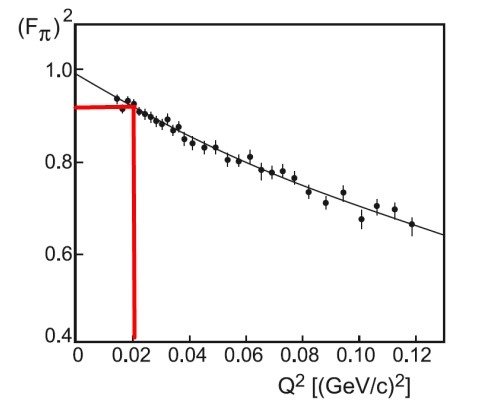
\includegraphics[width=0.7\textwidth]{Bilddateien/A1cGrafik.jpg}
                        \caption{Krasse Graffik alda}
                        \label{fig:A1cGrafik}
                \end{figure}

                

\end{document}